\documentclass{memoir}
\usepackage{amsmath}
\usepackage{amssymb}
\usepackage[utf8]{inputenc}
\usepackage{commath}
\usepackage{hyperref}
\usepackage{siunitx}
\usepackage{float}
\usepackage{graphicx}
\usepackage[left=2cm, top=2cm]{geometry}
\usepackage{pgfplotstable}
\usepackage{array}
\usepackage{cleveref}
\usepackage{wrapfig}
\title{Sine integral}
\date{}
\begin{document}
\section*{Sine integral}
\begin{wrapfigure}{r}{0.5\textwidth}
	% GNUPLOT: LaTeX picture with Postscript
\begingroup
  \makeatletter
  \providecommand\color[2][]{%
    \GenericError{(gnuplot) \space\space\space\@spaces}{%
      Package color not loaded in conjunction with
      terminal option `colourtext'%
    }{See the gnuplot documentation for explanation.%
    }{Either use 'blacktext' in gnuplot or load the package
      color.sty in LaTeX.}%
    \renewcommand\color[2][]{}%
  }%
  \providecommand\includegraphics[2][]{%
    \GenericError{(gnuplot) \space\space\space\@spaces}{%
      Package graphicx or graphics not loaded%
    }{See the gnuplot documentation for explanation.%
    }{The gnuplot epslatex terminal needs graphicx.sty or graphics.sty.}%
    \renewcommand\includegraphics[2][]{}%
  }%
  \providecommand\rotatebox[2]{#2}%
  \@ifundefined{ifGPcolor}{%
    \newif\ifGPcolor
    \GPcolortrue
  }{}%
  \@ifundefined{ifGPblacktext}{%
    \newif\ifGPblacktext
    \GPblacktexttrue
  }{}%
  % define a \g@addto@macro without @ in the name:
  \let\gplgaddtomacro\g@addto@macro
  % define empty templates for all commands taking text:
  \gdef\gplbacktext{}%
  \gdef\gplfronttext{}%
  \makeatother
  \ifGPblacktext
    % no textcolor at all
    \def\colorrgb#1{}%
    \def\colorgray#1{}%
  \else
    % gray or color?
    \ifGPcolor
      \def\colorrgb#1{\color[rgb]{#1}}%
      \def\colorgray#1{\color[gray]{#1}}%
      \expandafter\def\csname LTw\endcsname{\color{white}}%
      \expandafter\def\csname LTb\endcsname{\color{black}}%
      \expandafter\def\csname LTa\endcsname{\color{black}}%
      \expandafter\def\csname LT0\endcsname{\color[rgb]{1,0,0}}%
      \expandafter\def\csname LT1\endcsname{\color[rgb]{0,1,0}}%
      \expandafter\def\csname LT2\endcsname{\color[rgb]{0,0,1}}%
      \expandafter\def\csname LT3\endcsname{\color[rgb]{1,0,1}}%
      \expandafter\def\csname LT4\endcsname{\color[rgb]{0,1,1}}%
      \expandafter\def\csname LT5\endcsname{\color[rgb]{1,1,0}}%
      \expandafter\def\csname LT6\endcsname{\color[rgb]{0,0,0}}%
      \expandafter\def\csname LT7\endcsname{\color[rgb]{1,0.3,0}}%
      \expandafter\def\csname LT8\endcsname{\color[rgb]{0.5,0.5,0.5}}%
    \else
      % gray
      \def\colorrgb#1{\color{black}}%
      \def\colorgray#1{\color[gray]{#1}}%
      \expandafter\def\csname LTw\endcsname{\color{white}}%
      \expandafter\def\csname LTb\endcsname{\color{black}}%
      \expandafter\def\csname LTa\endcsname{\color{black}}%
      \expandafter\def\csname LT0\endcsname{\color{black}}%
      \expandafter\def\csname LT1\endcsname{\color{black}}%
      \expandafter\def\csname LT2\endcsname{\color{black}}%
      \expandafter\def\csname LT3\endcsname{\color{black}}%
      \expandafter\def\csname LT4\endcsname{\color{black}}%
      \expandafter\def\csname LT5\endcsname{\color{black}}%
      \expandafter\def\csname LT6\endcsname{\color{black}}%
      \expandafter\def\csname LT7\endcsname{\color{black}}%
      \expandafter\def\csname LT8\endcsname{\color{black}}%
    \fi
  \fi
    \setlength{\unitlength}{0.0500bp}%
    \ifx\gptboxheight\undefined%
      \newlength{\gptboxheight}%
      \newlength{\gptboxwidth}%
      \newsavebox{\gptboxtext}%
    \fi%
    \setlength{\fboxrule}{0.5pt}%
    \setlength{\fboxsep}{1pt}%
\begin{picture}(3960.00,2820.00)%
    \gplgaddtomacro\gplbacktext{%
      \csname LTb\endcsname%%
      \put(561,372){\makebox(0,0)[r]{\strut{}$-2$}}%
      \csname LTb\endcsname%%
      \put(561,608){\makebox(0,0)[r]{\strut{}$-1.5$}}%
      \csname LTb\endcsname%%
      \put(561,844){\makebox(0,0)[r]{\strut{}$-1$}}%
      \csname LTb\endcsname%%
      \put(561,1080){\makebox(0,0)[r]{\strut{}$-0.5$}}%
      \csname LTb\endcsname%%
      \put(561,1317){\makebox(0,0)[r]{\strut{}$0$}}%
      \csname LTb\endcsname%%
      \put(561,1553){\makebox(0,0)[r]{\strut{}$0.5$}}%
      \csname LTb\endcsname%%
      \put(561,1789){\makebox(0,0)[r]{\strut{}$1$}}%
      \csname LTb\endcsname%%
      \put(561,2025){\makebox(0,0)[r]{\strut{}$1.5$}}%
      \csname LTb\endcsname%%
      \put(561,2261){\makebox(0,0)[r]{\strut{}$2$}}%
      \csname LTb\endcsname%%
      \put(663,186){\makebox(0,0){\strut{}$0$}}%
      \csname LTb\endcsname%%
      \put(1261,186){\makebox(0,0){\strut{}$5$}}%
      \csname LTb\endcsname%%
      \put(1859,186){\makebox(0,0){\strut{}$10$}}%
      \csname LTb\endcsname%%
      \put(2457,186){\makebox(0,0){\strut{}$15$}}%
      \csname LTb\endcsname%%
      \put(3055,186){\makebox(0,0){\strut{}$20$}}%
      \csname LTb\endcsname%%
      \put(3653,186){\makebox(0,0){\strut{}$25$}}%
    }%
    \gplgaddtomacro\gplfronttext{%
      \csname LTb\endcsname%%
      \put(2158,2540){\makebox(0,0){\strut{}Sine integrals}}%
      \csname LTb\endcsname%%
      \put(2865,725){\makebox(0,0)[r]{\strut{}Si(x)}}%
      \csname LTb\endcsname%%
      \put(2865,539){\makebox(0,0)[r]{\strut{}si(x)}}%
    }%
    \gplbacktext
    \put(0,0){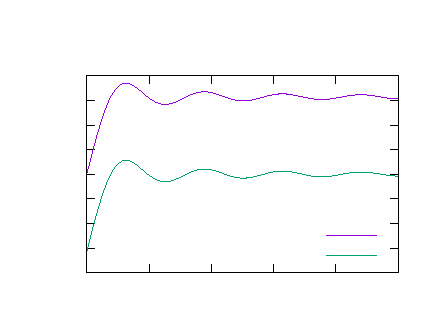
\includegraphics{SinIntPlot}}%
    \gplfronttext
  \end{picture}%
\endgroup

\end{wrapfigure}
The sine integral is part of the trigonometric integrals. It is defined in the following two ways 
\begin{align*}
	\mathrm{Si}(x)&=\int_{0}^{x}\frac{\sin t}{t}\dif x\\
	\mathrm{si}(x)&=-\int_{x}^{\infty}\frac{\sin t}{t}\dif x
\end{align*}
Both integrals are antiderivatives of the sinc function $\frac{\sin x}{x}$, but pertaining to different limits of the sinc function, as $\mathrm{Si}(x)$ is the antiderivative whose limit is $0$ as $x\rightarrow 0$, while $\mathrm{si}$ is the antiderivative whose value is $0$ as $x\rightarrow\infty$.
The integrals are related to each other by the integral \ref{Dirichlet}, the proof for which can be seen in \nameref{DirProof}
\begin{align}
	\label{Dirichlet}
	\mathrm{Si}(x)-\mathrm{si}(x)&=\int_{0}^{\infty}\frac{\sin t}{t}\dif t=\frac{\pi}{2}
\end{align}
This property is important when implementing the \textit{quad} integration routines, as the infinite integral of the \textit{Sin} function in $C\#$ takes an enormous amount of time.\\
Furthermore, for very large arguments ($x>700$), the solution exhibits sudden noise, uncharacteristic of the actual function. To avoid this, the functions were modified such that $\mathrm{Si}(x>700)=\frac{\pi}{2}$ and $\mathrm{si}(x>700)=0$, as the are already reasonably close to these values at this point.




\appendix
\section*{Appendix A}
\label{DirProof}
Starting with equation \ref{Dirichlet}, it is rewritten into a function of the variable $a$
\begin{align*}
	f(a)&=\int_{0}^{\infty}e^{-at}\frac{\sin t}{t}\dif t
\end{align*}
Where the particular integral used is $f(0)$.
The, utilizing Feynman's trick, we differentiate with respect to $a$
\begin{align*}
	\od{}{a}f&=\od{}{a}\int_{0}^{\infty} e^{-at}\frac{\sin t}{t}\dif t = \int_{0}^{\infty} \pd{}{a}e^{-at}\frac{\sin t}{t}\dif t = -\int_{0}^{\infty} e^{-at}\sin t \dif t
\end{align*}
Then rewriting with $\sin t = -\frac{1}{2i}\big(e^{it}-e^{-it}\big)$
\begin{align*}
	\od{f}{a}&=-\int_{0}^{\infty}e^{-at} \,\frac{e^{it}-e^{-it}}{21}\dif t=\frac{1}{2i}\int_{0}^{\infty}e^{-(a+i)t}-e^{-(a-i)t}\dif t\\
	&= \frac{1}{2i}\Big[ \frac{1}{a-i}e^{-(a-i)t}-\frac{1}{a+i}e^{-(a+i)t}  \Big]_0^{\infty}=-\frac{1}{1+a^2}
\end{align*}
Then applying integration
\begin{align*}
	f=\int \od{f}{a}\dif a=-\int \frac{1}{1+a^2}\dif a=-\arctan a + C
\end{align*}
Determining the integration constant $C$ from limit requirements
\begin{align*}
	\lim_{a\rightarrow \infty}f&=0=\lim_{a\rightarrow \infty}(C-\arctan a)\implies\\
	C&=\lim_{a\rightarrow \infty}\arctan a = \frac{\pi}{2}
\end{align*}
Such that
\begin{align*}
	f(a)= \frac{\pi}{2}-\arctan &a = \int_{0}^{\infty}e^{-at}\frac{\sin t}{t}\dif t\implies\\
	\int_{0}^{\infty}\frac{\sin t}{t}\dif t &= f(0) = \frac{\pi}{2}
\end{align*}



\end{document}
